% ------------------------------------------------------------------------------
% TYPO3 CMS 8.1 - What's New (English Version)
%
% @author	Patrick Lobacher <patrick@lobacher.de> and Michael Schams <schams.net>
% @license	Creative Commons BY-NC-SA 3.0
% @link		http://typo3.org/download/release-notes/whats-new/
% @language	English
% ------------------------------------------------------------------------------
% LTXE-CHAPTER-UID:		dcfe6009-2200ad81-816c2edb-1f54c687
% LTXE-CHAPTER-NAME:	Backend User Interface
% ------------------------------------------------------------------------------

\section{Gebruikersinterface backend}
\begin{frame}[fragile]
	\frametitle{Gebruikersinterface backend}

	\begin{center}\huge{Hoofdstuk 1:}\end{center}
	\begin{center}\huge{\color{typo3darkgrey}\textbf{Gebruikersinterface backend}}\end{center}

\end{frame}

% ------------------------------------------------------------------------------
% LTXE-SLIDE-START
% LTXE-SLIDE-UID:		a6e8ab9c-4ddc2807-90093bdb-5385b9bb
% LTXE-SLIDE-ORIGIN:	5d3d70fa-92a2935e-f1cbdc1e-285ec842 English
% LTXE-SLIDE-TITLE:		Feature: #75497 - inline backend layout wizard
% LTXE-SLIDE-REFERENCE:	!Feature-75497-InlineBackendLayoutWizard.rst
% ------------------------------------------------------------------------------
\begin{frame}[fragile]
	\frametitle{Gebruikersinterface backend}
	\framesubtitle{Inline Backend-lay-outAssistent}

	Een nieuw rendertype is toegevoegd om de backend-lay-outassistent in het formulier van de
	FormEngine af te beelden (in TCA: \texttt{'renderType' => 'belayoutwizard'}).

	\begin{figure}
		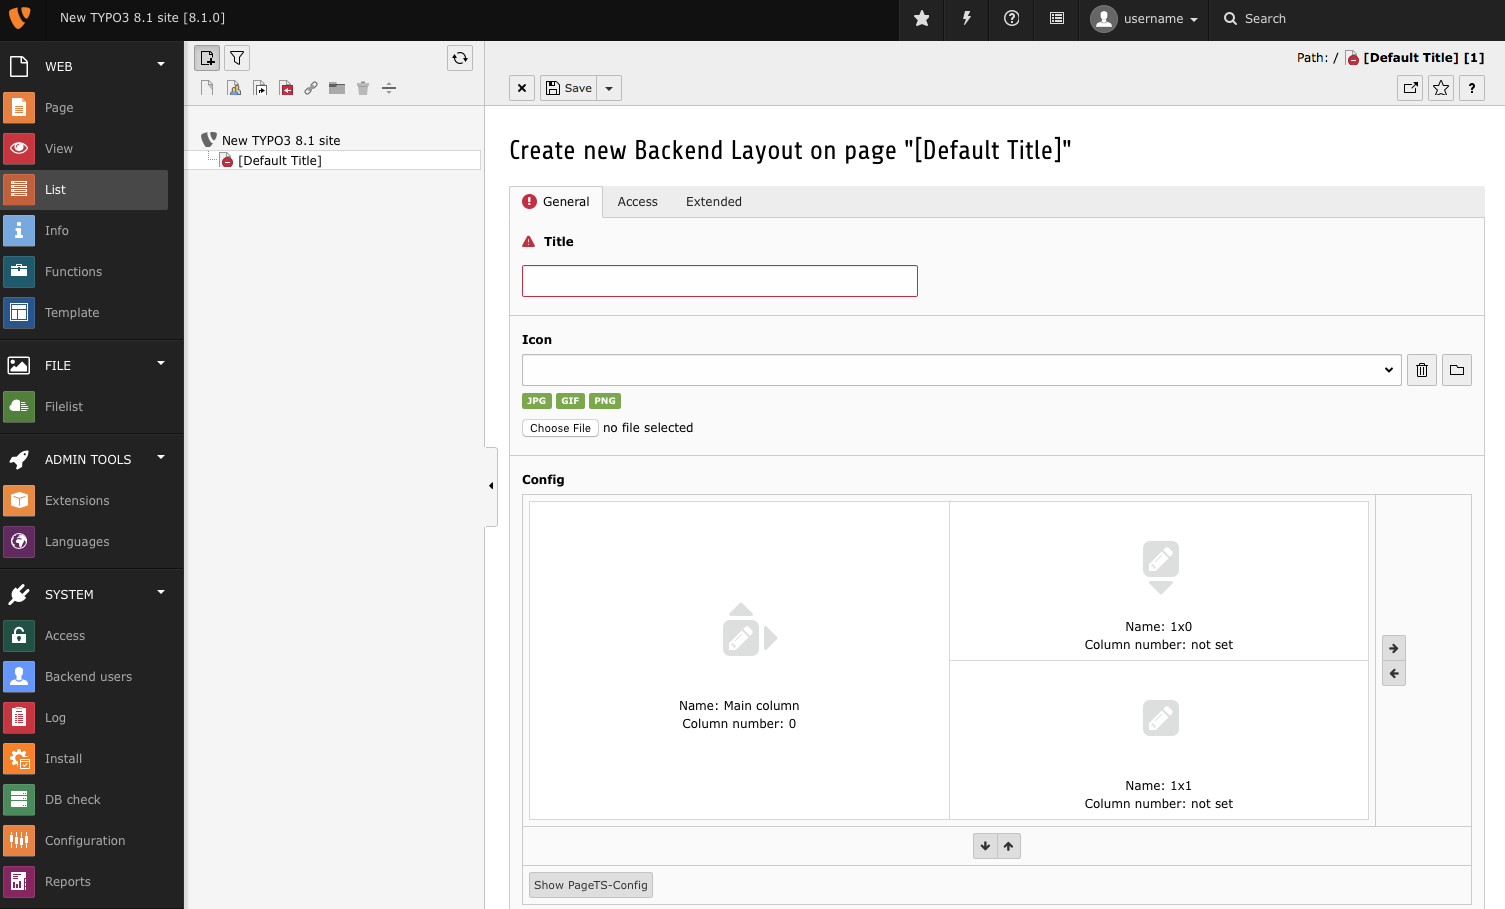
\includegraphics[width=0.70\linewidth]{BackendUserInterface/75497.png}
	\end{figure}

\end{frame}


% ------------------------------------------------------------------------------
% LTXE-SLIDE-START
% LTXE-SLIDE-UID:		10d47585-fca42c8f-2ceb3de6-40e8350a
% LTXE-SLIDE-ORIGIN:	7cab4dc0-cdfe9472-a3f0a874-dddf137d English
% LTXE-SLIDE-TITLE:		Feature: #75581 - Simplify cache clearing
% LTXE-SLIDE-REFERENCE:	!Feature-75581-SimplifyCacheClearing.rst
% ------------------------------------------------------------------------------
\begin{frame}[fragile]
	\frametitle{Gebruikersinterface backend}
	\framesubtitle{Eenvoudiger cahes legen}

	Het systeem om caches te legen is versimpeld door opties uit het cache-legen-menu en de
	Install Tool te verwijderen.

	\begin{itemize}

		\item \textbf{Frontend caches legen:}\newline
			\small
				Leegt frontend en paginagerelateerde caches, zoals eerder.
			\normalsize

		\item \textbf{Alle caches legen:}\newline
			\small
				Leegt alle systeemgerelateerde caches, waaronder de klasselader, vertalingen,
				cache voor de extensieconfiguratiebestanden, opcode cache. Het vernieuwen van
				deze cache kost wat tijd.
			\normalsize

	\end{itemize}

	\begin{figure}
		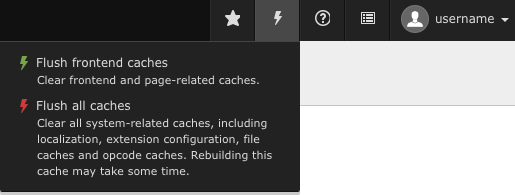
\includegraphics[width=0.45\linewidth]{BackendUserInterface/75581.png}
	\end{figure}

\end{frame}

% ------------------------------------------------------------------------------
% LTXE-SLIDE-START
% LTXE-SLIDE-UID:		246bf31b-76fa9b0b-6b70f1eb-b7671df1
% LTXE-SLIDE-ORIGIN:	e24e593c-fe9bcff9-c386db3a-79491de1 English
% LTXE-SLIDE-TITLE:		Rework Workspaces (1)
% LTXE-SLIDE-REFERENCE:	Rework Workspaces
% ------------------------------------------------------------------------------
\begin{frame}[fragile]
	\frametitle{Gebruikersinterface backend}
	\framesubtitle{Werkruimtes verbouwd (1)}

	\begin{itemize}

		\item De module Werkruimtes om klaargezette content te beheren is herschreven
		 	en past veel beter in het uiterlijk van de huidige backend

		\item Redacteuren zien direct dat het past bij de look-en-feel doordat het
		 	is gebaseerd op Twitter Bootstrap en jQuery

		\item De performance is hierdoor ook verbeterd. Het is een sprong voorwaarts
		 	naar een schonere en snellere TYPO3 backend met minder JavaScript

	\end{itemize}

\end{frame}

% ------------------------------------------------------------------------------
% LTXE-SLIDE-START
% LTXE-SLIDE-UID:		6519019a-62c792e8-80642aa1-de95d35f
% LTXE-SLIDE-ORIGIN:	fe9bcff9-e24e593c-79491de1-c386db3a English
% LTXE-SLIDE-TITLE:		Rework Workspaces (2)
% LTXE-SLIDE-REFERENCE:	Rework Workspaces
% ------------------------------------------------------------------------------
\begin{frame}[fragile]
	\frametitle{Gebruikersinterface backend}
	\framesubtitle{Werkruimtes verbouwd (2)}

	Schermafdrukken van de module werkruimtes:

	\begin{figure}
		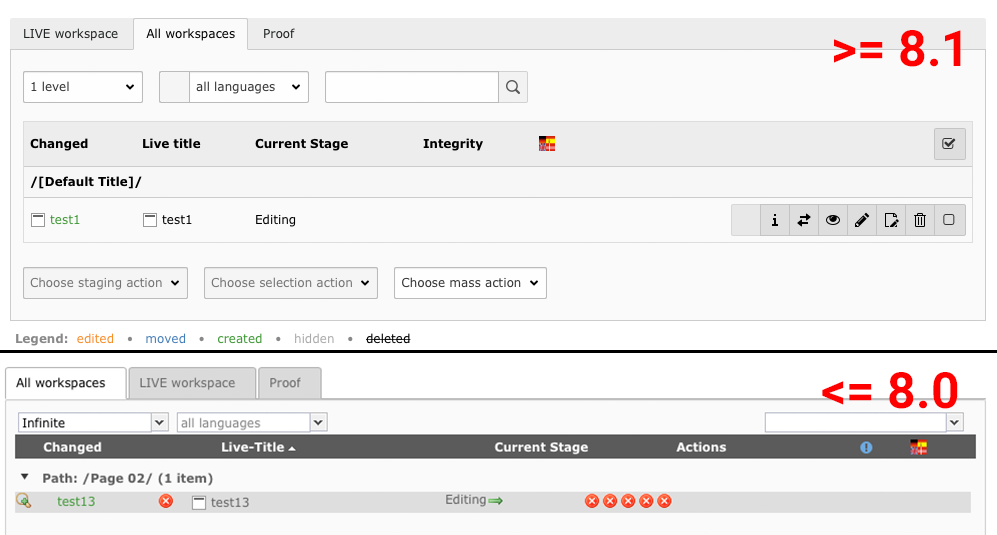
\includegraphics[width=0.85\linewidth]{BackendUserInterface/workspaces.png}
	\end{figure}

\end{frame}

% ------------------------------------------------------------------------------
